\documentclass[aspectratio=169]{beamer}
\usepackage{listings}
\newcommand\blank[1]{\rule[-.2ex]{#1}{.4pt}}
\usepackage{tikz}
\usepackage{fontawesome6}
\usepackage{url}
\usetikzlibrary{fit,backgrounds}
\usetikzlibrary{shapes.callouts, positioning, arrows.meta,calc}
\usetikzlibrary{decorations}
\usetikzlibrary{decorations.text}
\usetikzlibrary{decorations.pathreplacing}

\usepackage[dvipsnames]{xcolor}

\newcommand{\boxabstract}[2][fill=white]{
    \begin{center}
      \begin{tikzpicture}
        \node [abstractbox, #1] (box)
        {\begin{minipage}{0.80\linewidth}
%            \setlength{\parindent}{2mm}
            \footnotesize #2
          \end{minipage}};
        \node[abstracttitle, right=10pt] at (box.north west) {Stack};
      \end{tikzpicture}
    \end{center}
  }

% Use plain theme with no decorations
\usetheme{default}
\setbeamertemplate{navigation symbols}{}
\setbeamertemplate{footline}{}
\setbeamertemplate{headline}{}

% Define Java code style
\lstdefinestyle{JavaStyle}{
    language=Java,
    basicstyle=\ttfamily\tiny,
    keywordstyle=\color{blue}\bfseries,
    commentstyle=\color{green!60!black},
    stringstyle=\color{Maroon},
    numbers=left,
    numberstyle=\tiny\color{gray},
    stepnumber=1,
    numbersep=10pt,
    breaklines=true,
    frame=single,
    tabsize=2,
    showstringspaces=false,
    firstnumber=auto
}

\title{Comprendre l'évolution du stack en Java}
\subtitle{Semaine 4}
\author{École des Sciences Criminelles - UNIL}
\date{}

\begin{document}

\begin{frame}
\titlepage
\end{frame}

\begin{frame}{Terminologie}
    On utilise:
    \begin{itemize}
        \item $retAddr$ pour indiquer l'adresse de retour d'une méthode (return address).
        \item $retVal$ pour indiquer la valeur de retour d'une méthode (return value).
    \end{itemize}
\vspace{1cm}
On écrit de cette façon afin de rendre les choses plus explicites. Cependant, quand vous dessinez un diagramme du stack, il faut utiliser les conventions dans les diapositives du cours, c'est à dire:
\vspace{1cm}
\begin{itemize}
    \item 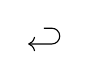
\begin{tikzpicture}[scale=0.1]
        \draw[->] (2,0) -- (3,0)
            to[out=0,in=90] (4,-1)
            to[out=-90,in=0] (3,-2)
            -- (0,-2);
    \end{tikzpicture} pour l'adresse de retour.
    \item 
\begin{tikzpicture}
        \draw[->, thick] (-0.5,0) -- (-0.5,0.3); 
    \end{tikzpicture} pour la valeur de retour.
\end{itemize}
\end{frame}

% \begin{frame}[fragile]{Code and Stack}
% \begin{columns}[T]
%     % Left column: Code with spotlight
%     \column{0.63\textwidth}
%     \begin{tikzpicture}
%         % Code listing (named node so we can reference its bounds)
%         \node[anchor=north west] (code) at (0,0) {
%             \begin{minipage}{\textwidth}
%     \begin{lstlisting}[style=JavaStyle,firstnumber=11]
    
%     }

%     public static void main(String[] args) {
%         int year = 2000;
%         reportLeapYear(year);
%     \end{lstlisting}
%             \end{minipage}
%         };
        
%         % === Spotlight the current line: draw a semi-opaque overlay with a hole ===
%         \begin{scope}[on background layer]
%             % Compute a window rectangle around the current line
%             \path let \p1=(code.north west), \p2=(code.north east) in
%                 coordinate (winNW) at (\x1, \y1-2.9em)  % top-left of the window
%                 coordinate (winSE) at (\x2, \y1-3.6em); % bottom-right of the window
            
%             % Wash out (pseudo-blur) everything except the window using even-odd rule
%             \fill[black,opacity=0.5,even odd rule]
%                 (code.south west) rectangle (code.north east)
%                 (winNW) rectangle (winSE);
            
%             % Draw the red box around the visible line
%             \draw[red,very thick,rounded corners=2pt] (winNW) rectangle (winSE);
%         \end{scope}
%     \end{tikzpicture}
    
%     % Right column: Stack diagram
%     \column{0.32\textwidth}
%     % \begin{tikzpicture}[font=\sffamily, scale=0.5]
%     %   % Draw the stack rectangles
%     %   \draw (0,0.0) rectangle (4.0,-1.0);
%     %   \draw (0,-1.0) rectangle (4.0,-2.0);
%     %   \draw (0,-2.0) rectangle (4.0,-3.0);
%     %   \draw (0,-3.0) rectangle (4.0,-4.0);
%     %   \draw (0,-4.0) rectangle (4.0,-5.0);
    
%     %   % Fill gray areas
%     %   \fill[gray!50] (0,-1.0) rectangle (4.0,-2.0);
%     %   \fill[gray!50] (0,-4.0) rectangle (4.0,-5.0);
    
%     %   % Labels inside rectangles
%     %   \node at (2.0,-0.5) {42};
%     %   \node at (2.0,-1.5) {10};
%     %   \node at (2.0,-2.5) {32};
%     %   \node at (2.0,-3.5) {0};
%     %   \node at (2.0,-4.5) {};
    
%     %   % Variable names on left
%     %   \node[anchor=east, text=red!70!black, font=\bfseries] at (0,-0.5) {result};
%     %   \node[anchor=east, text=red!70!black, font=\bfseries] at (0,-1.5) {x};
%     %   \node[anchor=east, text=red!70!black, font=\bfseries] at (0,-2.5) {y};
%     %   \node[anchor=east, text=red!70!black, font=\bfseries] at (0,-3.5) {temp};
    
%     %   % Bracket for annotation
%     %   % \draw[decorate,decoration={brace,amplitude=5pt,mirror}]
%     %   %   (4.0,-5.0) -- (4.0,0) node[midway,xshift=2.2cm,text width=3.5cm,align=left]
%     %   %   {stack frame of \\ \textit{\textbf{\textcolor{blue}{calculate}}} function};
%     % \end{tikzpicture}
% \end{columns}
% \vspace{1cm}
% On commence toujours l'exécution dans la méthode \texttt{main}!

% \end{frame}

% slide 2
% \begin{frame}[fragile]{\texttt{main}}
% \begin{columns}[T]
%     % Left column: Code with spotlight
%     \column{0.63\textwidth}
%     \begin{tikzpicture}
%         % Code listing (named node so we can reference its bounds)
%         \node[anchor=north west] (code) at (0,0) {
%             \begin{minipage}{\textwidth}
%     \begin{lstlisting}[style=JavaStyle,firstnumber=11]
    
%     }

%     public static void main(String[] args) {
%         int year = 2000;
%         reportLeapYear(year);
%     \end{lstlisting}
%             \end{minipage}
%         };
        
%         % === Spotlight the current line: draw a semi-opaque overlay with a hole ===
%         \begin{scope}[on background layer]
%             % Compute a window rectangle around the current line
%             \path let \p1=(code.north west), \p2=(code.north east) in
%                 coordinate (winNW) at (\x1, \y1-2.9em)  % top-left of the window
%                 coordinate (winSE) at (\x2, \y1-3.6em); % bottom-right of the window
            
%             % Wash out (pseudo-blur) everything except the window using even-odd rule
%             \fill[black,opacity=0.5,even odd rule]
%                 (code.south west) rectangle (code.north east)
%                 (winNW) rectangle (winSE);
            
%             % Draw the red box around the visible line
%             \draw[red,very thick,rounded corners=2pt] (winNW) rectangle (winSE);
%         \end{scope}
%     \end{tikzpicture}
    
%     % Right column: Stack diagram
%     \column{0.32\textwidth}
%     \begin{tikzpicture}[font=\sffamily, scale=0.5]
%   % Draw the stack rectangles
%   \draw (0,0.0) rectangle (4.0,-1.0);
%   \draw (0,-1.0) rectangle (4.0,-2.0);

%   % Fill gray areas
%   \fill[gray!50] (0,0.0) rectangle (4.0,-1.0);
%   \fill[gray!50] (0,-1.0) rectangle (4.0,-2.0);

%   % Labels inside rectangles
%   \node at (2.0,-0.5) {};
%   \node at (2.0,-1.5) {};

%   % Variable names on left
%   \node[anchor=east, text=red!70!black, font=\bfseries] at (-0.5,-0.5) {\footnotesize $retValue_{main}$};
%   \node[anchor=east, text=red!70!black, font=\bfseries] at (-0.5,-1.5) {\footnotesize $retAddr_{main}$};

%   % Arrows on left side
%   \draw[->, thick] (-0.3,-1.1) arc(70:-140:0.35);
%   \draw[->, thick] (-0.5,-0.8) -- (-0.5,-0.2);

%   % Bracket for annotation
%   \draw[decorate,decoration={brace,amplitude=5pt,mirror}]
%     (4.0,-2.0) -- (4.0,0) node[midway,xshift=2.2cm,text width=3.5cm,align=left]
%     {\tiny stack frame \\ \textit{\textbf{\textcolor{blue}{\tiny calculate}}} };

% \end{tikzpicture}
% \end{columns}
% \vspace{1cm}
% L'adresse de retour de la méthode \texttt{main} est dans le JVM \faCubes

% \end{frame}











% slide 3
\begin{frame}[fragile]{\texttt{main} (aucun argument de la ligne de commande)}
\begin{columns}[T]
    % Left column: Code with spotlight
    \column{0.63\textwidth}
    \begin{tikzpicture}
        % Code listing (named node so we can reference its bounds)
        \node[anchor=north west] (code) at (0,0) {
            \begin{minipage}{\textwidth}
    \begin{lstlisting}[style=JavaStyle,firstnumber=1]
public class LeapYear {
    static boolean isLeap(int year) {
        return (year % 4 == 0) && (year % 100 != 0) || (year % 400 == 0);
    }
    static void reportLeapYear(int year) {
        boolean leap = isLeap(year);
        System.out.println("isLeap(" + year + ")=" + leap);
    }
    public static void main(String[] args) {
        int year = 2000;
        reportLeapYear(year);
    }
}
    \end{lstlisting}
            \end{minipage}
        };
        
        % === Spotlight the current line: draw a semi-opaque overlay with a hole ===
        \begin{scope}[on background layer]
            % Compute a window rectangle around the current line
            \path let \p1=(code.north west), \p2=(code.north east) in
                coordinate (winNW) at (\x1, \y1-7.3em)  % top-left of the window
                coordinate (winSE) at (\x2, \y1-6.6em); % bottom-right of the window
            
            % Wash out (pseudo-blur) everything except the window using even-odd rule
            \fill[black,opacity=0.3,even odd rule]
                ([yshift=0.33cm]code.south west) rectangle ([yshift=-0.27cm]code.north east)
                (winNW) rectangle (winSE);
            
            % Draw the red box around the visible line
            \draw[red,very thick,rounded corners=2pt] (winNW) rectangle (winSE);
        \end{scope}
    \end{tikzpicture}
    
    % Right column: Stack diagram
    \column{0.32\textwidth}
    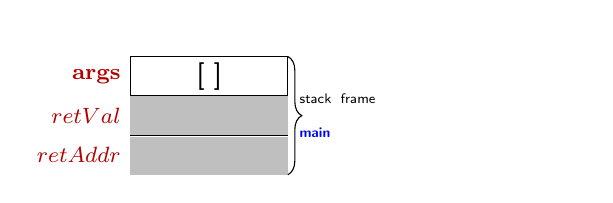
\begin{tikzpicture}[font=\sffamily, scale=0.5]
    % Draw the stack rectangles
  % \draw (0,0.0) rectangle (4.0,-1.0);
  \draw (0,-1.0) rectangle (4.0,-2.0);
  \draw (0,-2.0) rectangle (4.0,-3.0);
  \draw (0,-3.05) rectangle (4.0,-4.0);

  % Fill gray areas
  \fill[gray!50] (0,-2.0) rectangle (4.0,-3.0);
  \fill[gray!50] (0,-3.05) rectangle (4.0,-4.0);

  % Labels inside rectangles
  \node at (2.0,-0.5) {};
  \node at (2.0,-1.5) {[\ ]};
  \node at (2.0,-2.5) {};
  \node at (2.0,-3.5) {};


  \node[anchor=east, text=red!70!black, font=\bfseries] at (0,-1.5) {\footnotesize args};
 \node[anchor=east, text=red!70!black, font=\bfseries] at (0,-2.5) {\footnotesize $retVal$};
  \node[anchor=east, text=red!70!black, font=\bfseries] at (0,-3.5) {\footnotesize $retAddr$};

  % Arrows on left side
  % \draw[->, thick] (-0.3,-0.1) arc(70:-140:0.35);
  % \draw[->, thick] (-0.5,-1.8) -- (-0.5,-1.2);

  % Bracket for annotation
  
\draw[decorate,decoration={brace,amplitude=5pt,mirror}]
    (4.0,-4.0) -- (4.0,-1) node[midway,xshift=1.9cm,text width=3.5cm,align=left]
    {\tiny stack frame \\ \textit{\textbf{\textcolor{blue}{main}}} };

\end{tikzpicture}
\end{columns}
\vspace{1cm}
On commence toujours l'exécution dans la méthode \texttt{main}! \newline
L'adresse de retour de la méthode \texttt{main} est dans le JVM \faJava
\end{frame}

















% slide 4
\begin{frame}[fragile]{\texttt{main:L10}}
\begin{columns}[T]
    % Left column: Code with spotlight
    \column{0.63\textwidth}
    \begin{tikzpicture}
        % Code listing (named node so we can reference its bounds)
        \node[anchor=north west] (code) at (0,0) {
            \begin{minipage}{\textwidth}
    \begin{lstlisting}[style=JavaStyle,firstnumber=1]
public class LeapYear {
    static boolean isLeap(int year) {
        return (year % 4 == 0) && (year % 100 != 0) || (year % 400 == 0);
    }
    static void reportLeapYear(int year) {
        boolean leap = isLeap(year);
        System.out.println("isLeap(" + year + ")=" + leap);
    }
    public static void main(String[] args) {
        int year = 2000;
        reportLeapYear(year);
    }
}
    \end{lstlisting}
            \end{minipage}
        };
        
        % === Spotlight the current line: draw a semi-opaque overlay with a hole ===
        \begin{scope}[on background layer]
            % Compute a window rectangle around the current line
            \path let \p1=(code.north west), \p2=(code.north east) in
                coordinate (winNW) at (\x1, \y1-8em)  % top-left of the window
                coordinate (winSE) at (\x2, \y1-7.3em); % bottom-right of the window
            
            % Wash out (pseudo-blur) everything except the window using even-odd rule
            \fill[black,opacity=0.3,even odd rule]
                ([yshift=0.34cm]code.south west) rectangle ([yshift=-0.27cm]code.north east)
                (winNW) rectangle (winSE);
            
            % Draw the red box around the visible line
            \draw[red,very thick,rounded corners=2pt] (winNW) rectangle (winSE);
        \end{scope}
    \end{tikzpicture}
    
    % Right column: Stack diagram
    \column{0.32\textwidth}
    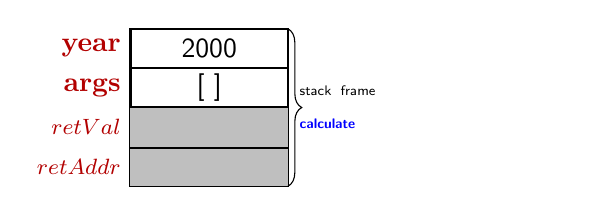
\begin{tikzpicture}[font=\sffamily, scale=0.5]
    % Draw the stack rectangles
  \draw[thick] (0,0.0) rectangle (4.0,-1.0);
  \draw[thick] (0,-1.0) rectangle (4.0,-2.0);
  \draw[thick] (0,-2.0) rectangle (4.0,-3.0);
  \draw[thick] (0,-3.05) rectangle (4.0,-4.0);

  % Fill gray areas
  \fill[gray!50] (0,-2.0) rectangle (4.0,-3.0);
  \fill[gray!50] (0,-3.05) rectangle (4.0,-4.0);

  % Labels inside rectangles
  \node at (2.0,-0.5) {2000};
  \node at (2.0,-1.5) {[\ ]};
  \node at (2.0,-2.5) {};
  \node at (2.0,-3.5) {};

  % Variable names on left
  \node[anchor=east, text=red!70!black, font=\bfseries] at (0,-0.5) {year};
  \node[anchor=east, text=red!70!black, font=\bfseries] at (0,-1.5) {args};
  \node[anchor=east, text=red!70!black, font=\bfseries] at (0,-2.5) {\footnotesize $retVal$};
  \node[anchor=east, text=red!70!black, font=\bfseries] at (0,-3.5) {\footnotesize $retAddr$};

  % Bracket for annotation
  \draw[decorate,decoration={brace,amplitude=5pt,mirror}]
    (4.0,-4.0) -- (4.0,0) node[midway,xshift=1.9cm,text width=3.5cm,align=left]
    {\tiny stack frame \\ \textit{\textbf{\textcolor{blue}{calculate}}} };
\end{tikzpicture}
\end{columns}
\vspace{1cm}

\end{frame}







% slide 5
\begin{frame}[fragile]{\texttt{main:L11}}
\begin{columns}[T]
    % Left column: Code with spotlight
    \column{0.63\textwidth}
    \begin{tikzpicture}
        % Code listing (named node so we can reference its bounds)
        \node[anchor=north west] (code) at (0,0) {
            \begin{minipage}{\textwidth}
    \begin{lstlisting}[style=JavaStyle,firstnumber=1]
public class LeapYear {
    static boolean isLeap(int year) {
        return (year % 4 == 0) && (year % 100 != 0) || (year % 400 == 0);
    }
    static void reportLeapYear(int year) {
        boolean leap = isLeap(year);
        System.out.println("isLeap(" + year + ")=" + leap);
    }
    public static void main(String[] args) {
        int year = 2000;
        reportLeapYear(year);
    }
}
    \end{lstlisting}
            \end{minipage}
        };
        
        % === Spotlight the current line: draw a semi-opaque overlay with a hole ===
        \begin{scope}[on background layer]
            % Compute a window rectangle around the current line
            \path let \p1=(code.north west), \p2=(code.north east) in
                coordinate (winNW) at (\x1, \y1-8.6em)  % top-left of the window
                coordinate (winSE) at (\x2, \y1-7.9em); % bottom-right of the window
            
            % Wash out (pseudo-blur) everything except the window using even-odd rule
            \fill[black,opacity=0.3,even odd rule]
                ([yshift=0.34cm]code.south west) rectangle ([yshift=-0.27cm]code.north east)
                (winNW) rectangle (winSE);
            
            % Draw the red box around the visible line
            \draw[red,very thick,rounded corners=2pt] (winNW) rectangle (winSE);
        \end{scope}
    \end{tikzpicture}
    
    % Right column: Stack diagram
    \column{0.32\textwidth}
    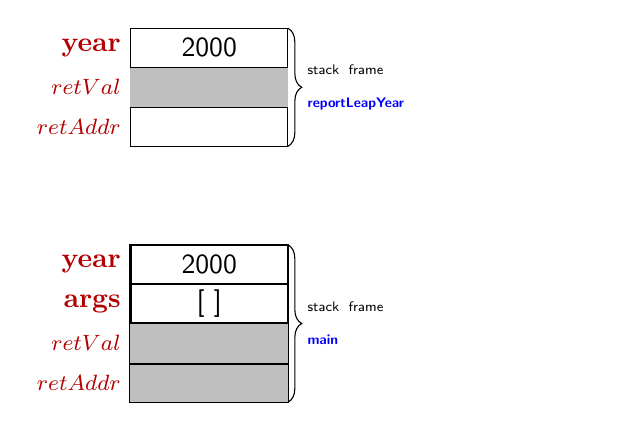
\begin{tikzpicture}[font=\sffamily, scale=0.5]
    \begin{scope}
      % Draw the stack rectangles

  \draw (0,-1.0) rectangle (4.0,-2.0);
  \draw (0,-2.0) rectangle (4.0,-3.0);
  \draw (0,-3.0) rectangle (4.0,-4.0);

  % Fill gray areas
  \fill[gray!50] (0,-2.0) rectangle (4.0,-3.0);

  % Labels inside rectangles

  \node at (2.0,-1.5) {2000};
  \node at (2.0,-2.5) {};
  \node at (2.0,-3.5) {};

  % Variable names on left

  \node[anchor=east, text=red!70!black, font=\bfseries] at (0,-1.5) {year};
  \node[anchor=east, text=red!70!black, font=\bfseries] at (0,-2.5) {\footnotesize $retVal$};
  \node[anchor=east, text=red!70!black, font=\bfseries] at (0,-3.5) {\footnotesize $retAddr$};

  % Bracket for annotation
  \draw[decorate,decoration={brace,amplitude=5pt,mirror}]
    (4.0,-4.0) -- (4.0,-1) node[midway,xshift=2cm,text width=3.5cm,align=left]
    {\tiny stack frame \\ \textit{\textbf{\textcolor{blue}{reportLeapYear}}}};
  \end{scope}

  % Second picture shifted down by 0.5 cm
  \begin{scope}[yshift=-6.5cm] % radius 1cm + 0.5cm gap
    % Draw the stack rectangles
  \draw[thick] (0,0.0) rectangle (4.0,-1.0);
  \draw[thick] (0,-1.0) rectangle (4.0,-2.0);
  \draw[thick] (0,-2.0) rectangle (4.0,-3.0);
  \draw[thick] (0,-3.05) rectangle (4.0,-4.0);

  % Fill gray areas
  \fill[gray!50] (0,-2.0) rectangle (4.0,-3.0);
  \fill[gray!50] (0,-3.05) rectangle (4.0,-4.0);

  % Labels inside rectangles
  \node at (2.0,-0.5) {2000};
  \node at (2.0,-1.5) {[\ ]};
  \node at (2.0,-2.5) {};
  \node at (2.0,-3.5) {};

  % Variable names on left
  \node[anchor=east, text=red!70!black, font=\bfseries] at (0,-0.5) {year};
  \node[anchor=east, text=red!70!black, font=\bfseries] at (0,-1.5) {args};
  \node[anchor=east, text=red!70!black, font=\bfseries] at (0,-2.5) {\footnotesize $retVal$};
  \node[anchor=east, text=red!70!black, font=\bfseries] at (0,-3.5) {\footnotesize $retAddr$};

  % Bracket for annotation
  \draw[decorate,decoration={brace,amplitude=5pt,mirror}]
    (4.0,-4.0) -- (4.0,0) node[midway,xshift=2cm,text width=3.5cm,align=left]
    {\tiny stack frame \\ \textit{\textbf{\textcolor{blue}{main}}} };
  \end{scope}
    % \
      
    \end{tikzpicture}
\end{columns}
\vspace{1cm}

\end{frame}












% slide 5
\begin{frame}[fragile]{\texttt{reportLeapYear}:L6 (allocation de la variable \texttt{leap})}
\begin{columns}[T]
    % Left column: Code with spotlight
    \column{0.63\textwidth}
    \begin{tikzpicture}
        % Code listing (named node so we can reference its bounds)
        \node[anchor=north west] (code) at (0,0) {
            \begin{minipage}{\textwidth}
   \begin{lstlisting}[style=JavaStyle,firstnumber=1]
public class LeapYear {
    static boolean isLeap(int year) {
        return (year % 4 == 0) && (year % 100 != 0) || (year % 400 == 0);
    }
    static void reportLeapYear(int year) {
        boolean leap = isLeap(year);
        System.out.println("isLeap(" + year + ")=" + leap);
    }
    public static void main(String[] args) {
        int year = 2000;
        reportLeapYear(year);
    }
}
    \end{lstlisting}
            \end{minipage}
        };
        
        % === Spotlight the current line: draw a semi-opaque overlay with a hole ===
        \begin{scope}[on background layer]
            % Compute a window rectangle around the current line
            \path let \p1=(code.north west), \p2=(code.north east) in
                coordinate (winNW) at (\x1, \y1-5.4em)  % top-left of the window
                coordinate (winSE) at (\x2, \y1-4.7em); % bottom-right of the window
            
            % Wash out (pseudo-blur) everything except the window using even-odd rule
            \fill[black,opacity=0.3,even odd rule]
                ([yshift=0.34cm]code.south west) rectangle ([yshift=-0.27cm]code.north east)
                (winNW) rectangle (winSE);
            
            % Draw the red box around the visible line
            \draw[red,very thick,rounded corners=2pt] (winNW) rectangle (winSE);
        \end{scope}
    \end{tikzpicture}
    
    % Right column: Stack diagram
    \column{0.32\textwidth}
    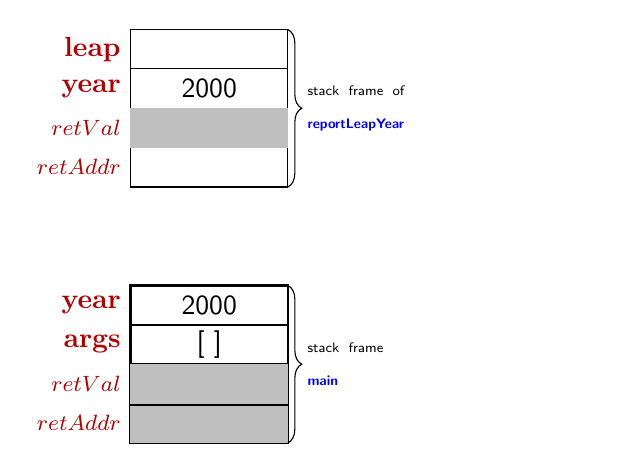
\begin{tikzpicture}[font=\sffamily, scale=0.5]
    \begin{scope}
      % Draw the stack rectangles
  \draw (0,-0.0) rectangle (4.0,-1.0);
  \draw (0,-1.0) rectangle (4.0,-2.0);
  \draw (0,-2.0) rectangle (4.0,-3.0);
  \draw (0,-3.0) rectangle (4.0,-4.0);

  % Fill gray areas
  \fill[gray!50] (0,-2.0) rectangle (4.0,-3.0);

  % Labels inside rectangles

  \node at (2.0,-1.5) {2000};
  \node at (2.0,-2.5) {};
  \node at (2.0,-3.5) {};

  % Variable names on left
  \node[anchor=east, text=red!70!black, font=\bfseries] at (0,-0.5) {leap};
  \node[anchor=east, text=red!70!black, font=\bfseries] at (0,-1.5) {year};
  \node[anchor=east, text=red!70!black, font=\bfseries] at (0,-2.5) {\footnotesize $retVal$};
  \node[anchor=east, text=red!70!black, font=\bfseries] at (0,-3.5) {\footnotesize $retAddr$};

  % Bracket for annotation
  \draw[decorate,decoration={brace,amplitude=5pt,mirror}]
    (4.0,-4.0) -- (4.0,0) node[midway,xshift=2cm,text width=3.5cm,align=left]
    {\tiny stack frame of \\ \textit{\textbf{\textcolor{blue}{reportLeapYear}}}};
  \end{scope}

  % Second picture shifted down by 0.5 cm
  \begin{scope}[yshift=-6.5cm] % radius 1cm + 0.5cm gap
    % Draw the stack rectangles
  \draw[thick] (0,0.0) rectangle (4.0,-1.0);
  \draw[thick] (0,-1.0) rectangle (4.0,-2.0);
  \draw[thick] (0,-2.0) rectangle (4.0,-3.0);
  \draw[thick] (0,-3.05) rectangle (4.0,-4.0);

  % Fill gray areas
  \fill[gray!50] (0,-2.0) rectangle (4.0,-3.0);
  \fill[gray!50] (0,-3.05) rectangle (4.0,-4.0);

  % Labels inside rectangles
  \node at (2.0,-0.5) {2000};
  \node at (2.0,-1.5) {[\ ]};
  \node at (2.0,-2.5) {};
  \node at (2.0,-3.5) {};

  % Variable names on left
  \node[anchor=east, text=red!70!black, font=\bfseries] at (0,-0.5) {year};
  \node[anchor=east, text=red!70!black, font=\bfseries] at (0,-1.5) {args};
  \node[anchor=east, text=red!70!black, font=\bfseries] at (0,-2.5) {\footnotesize $retVal$};
  \node[anchor=east, text=red!70!black, font=\bfseries] at (0,-3.5) {\footnotesize $retAddr$};

  % Bracket for annotation
  \draw[decorate,decoration={brace,amplitude=5pt,mirror}]
    (4.0,-4.0) -- (4.0,0) node[midway,xshift=2cm,text width=3.5cm,align=left]
    {\tiny stack frame \\ \textit{\textbf{\textcolor{blue}{main}}} };
  \end{scope}
    % \
      
    \end{tikzpicture}
\end{columns}
\vspace{1cm}

\end{frame}















% slide 5
\begin{frame}[fragile]{\texttt{reportLeapYear}:L6 (appel de la méthode \texttt{isLeap})}
\begin{columns}[T]
    % Left column: Code with spotlight
    \column{0.63\textwidth}
    \begin{tikzpicture}
        % Code listing (named node so we can reference its bounds)
        \node[anchor=north west] (code) at (0,0) {
            \begin{minipage}{\textwidth}
   \begin{lstlisting}[style=JavaStyle,firstnumber=1]
public class LeapYear {
    static boolean isLeap(int year) {
        return (year % 4 == 0) && (year % 100 != 0) || (year % 400 == 0);
    }
    static void reportLeapYear(int year) {
        boolean leap = isLeap(year);
        System.out.println("isLeap(" + year + ")=" + leap);
    }
    public static void main(String[] args) {
        int year = 2000;
        reportLeapYear(year);
    }
}
    \end{lstlisting}
            \end{minipage}
        };
        
        % === Spotlight the current line: draw a semi-opaque overlay with a hole ===
        \begin{scope}[on background layer]
            % Compute a window rectangle around the current line
            \path let \p1=(code.north west), \p2=(code.north east) in
                coordinate (winNW) at (\x1, \y1-5.4em)  % top-left of the window
                coordinate (winSE) at (\x2, \y1-4.7em); % bottom-right of the window
            
            % Wash out (pseudo-blur) everything except the window using even-odd rule
            \fill[black,opacity=0.3,even odd rule]
                ([yshift=0.34cm]code.south west) rectangle ([yshift=-0.27cm]code.north east)
                (winNW) rectangle (winSE);
            
            % Draw the red box around the visible line
            \draw[red,very thick,rounded corners=2pt] (winNW) rectangle (winSE);
        \end{scope}
    \end{tikzpicture}
    
    % Right column: Stack diagram
    \column{0.32\textwidth}
    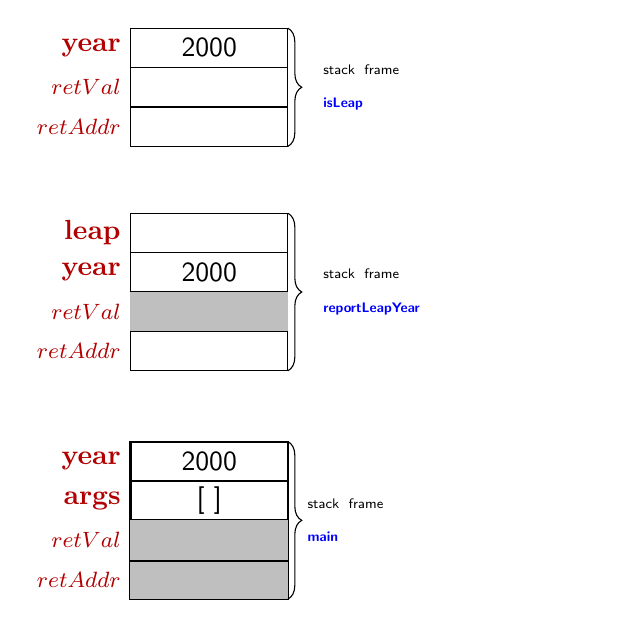
\begin{tikzpicture}[font=\sffamily, scale=0.5]
    \begin{scope}[yshift=4cm]
          % Draw the stack rectangles
  \draw (0,0.0) rectangle (4.0,-1.0);
  \draw (0,-1.0) rectangle (4.0,-2.0);
  \draw (0,-2.0) rectangle (4.0,-3.0);

  % Labels inside rectangles
  \node at (2.0,-0.5) {2000};
  \node at (2.0,-1.5) {};
  \node at (2.0,-2.5) {};

  % Variable names on left
  \node[anchor=east, text=red!70!black, font=\bfseries] at (0,-0.5) {year};
  \node[anchor=east, text=red!70!black, font=\bfseries] at (0,-1.5) {\footnotesize $retVal$};
  \node[anchor=east, text=red!70!black, font=\bfseries] at (0,-2.5) {\footnotesize $retAddr$};

  % Bracket for annotation
  \draw[decorate,decoration={brace,amplitude=5pt,mirror}]
    (4.0,-3.0) -- (4.0,0) node[midway,xshift=2.2cm,text width=3.5cm,align=left]
    {\tiny stack frame \\ \textit{\textbf{\textcolor{blue}{isLeap}}} };
    \end{scope}
    \begin{scope}[yshift=-0.7cm]
      % Draw the stack rectangles
  \draw (0,-0.0) rectangle (4.0,-1.0);
  \draw (0,-1.0) rectangle (4.0,-2.0);
  \draw (0,-2.0) rectangle (4.0,-3.0);
  \draw (0,-3.0) rectangle (4.0,-4.0);

  % Fill gray areas
  \fill[gray!50] (0,-2.0) rectangle (4.0,-3.0);

  % Labels inside rectangles

  \node at (2.0,-1.5) {2000};
  \node at (2.0,-2.5) {};
  \node at (2.0,-3.5) {};

  % Variable names on left
  \node[anchor=east, text=red!70!black, font=\bfseries] at (0,-0.5) {leap};
  \node[anchor=east, text=red!70!black, font=\bfseries] at (0,-1.5) {year};
  \node[anchor=east, text=red!70!black, font=\bfseries] at (0,-2.5) {\footnotesize $retVal$};
  \node[anchor=east, text=red!70!black, font=\bfseries] at (0,-3.5) {\footnotesize $retAddr$};

  % Bracket for annotation
  \draw[decorate,decoration={brace,amplitude=5pt,mirror}]
    (4.0,-4.0) -- (4.0,0) node[midway,xshift=2.2cm,text width=3.5cm,align=left]
    {\tiny stack frame \\ \textit{\textbf{\textcolor{blue}{reportLeapYear}}}};
  \end{scope}

  %   \begin{scope}
  %     % Draw the stack rectangles
  % \draw (0,-0.0) rectangle (4.0,-1.0);
  % \draw (0,-1.0) rectangle (4.0,-2.0);
  % \draw (0,-2.0) rectangle (4.0,-3.0);
  % \draw (0,-3.0) rectangle (4.0,-4.0);

  % % Fill gray areas
  % \fill[gray!50] (0,-2.0) rectangle (4.0,-3.0);

  % % Labels inside rectangles

  % \node at (2.0,-1.5) {2000};
  % \node at (2.0,-2.5) {};
  % \node at (2.0,-3.5) {};

  % % Variable names on left
  % \node[anchor=east, text=red!70!black, font=\bfseries] at (0,-0.5) {leap};
  % \node[anchor=east, text=red!70!black, font=\bfseries] at (0,-1.5) {year};
  % \node[anchor=east, text=red!70!black, font=\bfseries] at (0,-2.5) {\footnotesize $retVal$};
  % \node[anchor=east, text=red!70!black, font=\bfseries] at (0,-3.5) {\footnotesize $retAddr$};

  % % Bracket for annotation
  % \draw[decorate,decoration={brace,amplitude=5pt,mirror}]
  %   (4.0,-4.0) -- (4.0,0) node[midway,xshift=2cm,text width=3.5cm,align=left]
  %   {\tiny stack frame of \\ \textit{\textbf{\textcolor{blue}{reportLeapYear}}}};
  % \end{scope}

  % Second picture shifted down by 0.5 cm
  \begin{scope}[yshift=-6.5cm] % radius 1cm + 0.5cm gap
    % Draw the stack rectangles
  \draw[thick] (0,0.0) rectangle (4.0,-1.0);
  \draw[thick] (0,-1.0) rectangle (4.0,-2.0);
  \draw[thick] (0,-2.0) rectangle (4.0,-3.0);
  \draw[thick] (0,-3.05) rectangle (4.0,-4.0);

  % Fill gray areas
  \fill[gray!50] (0,-2.0) rectangle (4.0,-3.0);
  \fill[gray!50] (0,-3.05) rectangle (4.0,-4.0);

  % Labels inside rectangles
  \node at (2.0,-0.5) {2000};
  \node at (2.0,-1.5) {[\ ]};
  \node at (2.0,-2.5) {};
  \node at (2.0,-3.5) {};

  % Variable names on left
  \node[anchor=east, text=red!70!black, font=\bfseries] at (0,-0.5) {year};
  \node[anchor=east, text=red!70!black, font=\bfseries] at (0,-1.5) {args};
  \node[anchor=east, text=red!70!black, font=\bfseries] at (0,-2.5) {\footnotesize $retVal$};
  \node[anchor=east, text=red!70!black, font=\bfseries] at (0,-3.5) {\footnotesize $retAddr$};

  % Bracket for annotation
  \draw[decorate,decoration={brace,amplitude=5pt,mirror}]
    (4.0,-4.0) -- (4.0,0) node[midway,xshift=2cm,text width=3.5cm,align=left]
    {\tiny stack frame \\ \textit{\textbf{\textcolor{blue}{main}}} };
  \end{scope}
    % \
      
    \end{tikzpicture}
\end{columns}
\vspace{1cm}

\end{frame}













% slide 5
\begin{frame}[fragile]{\texttt{isLeap:L3}}
\begin{columns}[T]
    % Left column: Code with spotlight
    \column{0.63\textwidth}
    \begin{tikzpicture}
        % Code listing (named node so we can reference its bounds)
        \node[anchor=north west] (code) at (0,0) {
            \begin{minipage}{\textwidth}
   \begin{lstlisting}[style=JavaStyle,firstnumber=1]
public class LeapYear {
    static boolean isLeap(int year) {
        return (year % 4 == 0) && (year % 100 != 0) || (year % 400 == 0);
    }
    static void reportLeapYear(int year) {
        boolean leap = isLeap(year);
        System.out.println("isLeap(" + year + ")=" + leap);
    }
    public static void main(String[] args) {
        int year = 2000;
        reportLeapYear(year);
    }
}
    \end{lstlisting}
            \end{minipage}
        };
        
        % === Spotlight the current line: draw a semi-opaque overlay with a hole ===
        \begin{scope}[on background layer]
            % Compute a window rectangle around the current line
            \path let \p1=(code.north west), \p2=(code.north east) in
                coordinate (winNW) at (\x1, \y1-3.4em)  % top-left of the window
                coordinate (winSE) at (\x2, \y1-2.1em); % bottom-right of the window
            
            % Wash out (pseudo-blur) everything except the window using even-odd rule
            \fill[black,opacity=0.3,even odd rule]
                ([yshift=0.34cm]code.south west) rectangle ([yshift=-0.27cm]code.north east)
                (winNW) rectangle (winSE);
            
            % Draw the red box around the visible line
            \draw[red,very thick,rounded corners=2pt] (winNW) rectangle (winSE);
        \end{scope}
    \end{tikzpicture}
    
    % Right column: Stack diagram
    \column{0.32\textwidth}
    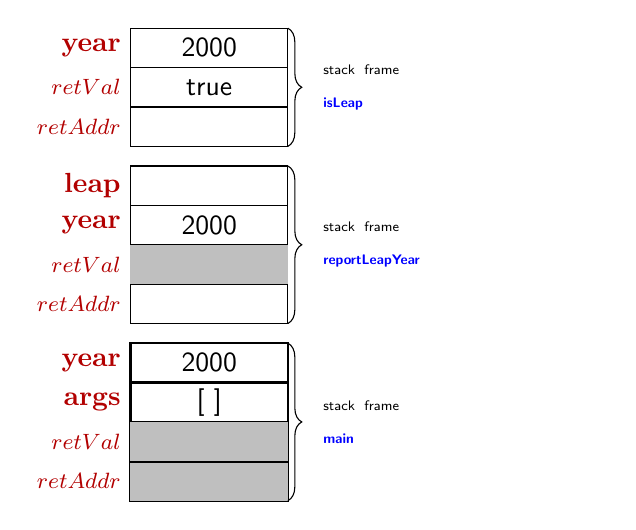
\begin{tikzpicture}[font=\sffamily, scale=0.5]
    \begin{scope}[yshift=2cm]
          % Draw the stack rectangles
  \draw (0,0.0) rectangle (4.0,-1.0);
  \draw (0,-1.0) rectangle (4.0,-2.0);
  \draw (0,-2.0) rectangle (4.0,-3.0);

  % Labels inside rectangles
  \node at (2.0,-0.5) {2000};
  \node at (2.0,-1.5) {true};
  \node at (2.0,-2.5) {};

  % Variable names on left
  \node[anchor=east, text=red!70!black, font=\bfseries] at (0,-0.5) {year};
  \node[anchor=east, text=red!70!black, font=\bfseries] at (0,-1.5) {\footnotesize $retVal$};
  \node[anchor=east, text=red!70!black, font=\bfseries] at (0,-2.5) {\footnotesize $retAddr$};

  % Bracket for annotation
  \draw[decorate,decoration={brace,amplitude=5pt,mirror}]
    (4.0,-3.0) -- (4.0,0) node[midway,xshift=2.2cm,text width=3.5cm,align=left]
    {\tiny stack frame \\ \textit{\textbf{\textcolor{blue}{isLeap}}}};
    \end{scope}
    \begin{scope}[yshift=-1.5cm]
      % Draw the stack rectangles
  \draw (0,-0.0) rectangle (4.0,-1.0);
  \draw (0,-1.0) rectangle (4.0,-2.0);
  \draw (0,-2.0) rectangle (4.0,-3.0);
  \draw (0,-3.0) rectangle (4.0,-4.0);

  % Fill gray areas
  \fill[gray!50] (0,-2.0) rectangle (4.0,-3.0);

  % Labels inside rectangles

  \node at (2.0,-1.5) {2000};
  \node at (2.0,-2.5) {};
  \node at (2.0,-3.5) {};

  % Variable names on left
  \node[anchor=east, text=red!70!black, font=\bfseries] at (0,-0.5) {leap};
  \node[anchor=east, text=red!70!black, font=\bfseries] at (0,-1.5) {year};
  \node[anchor=east, text=red!70!black, font=\bfseries] at (0,-2.5) {\footnotesize $retVal$};
  \node[anchor=east, text=red!70!black, font=\bfseries] at (0,-3.5) {\footnotesize $retAddr$};

  % Bracket for annotation
  \draw[decorate,decoration={brace,amplitude=5pt,mirror}]
    (4.0,-4.0) -- (4.0,0) node[midway,xshift=2.2cm,text width=3.5cm,align=left]
    {\tiny stack frame \\ \textit{\textbf{\textcolor{blue}{reportLeapYear}}}};
  \end{scope}

  % Second picture shifted down by 0.5 cm
  \begin{scope}[yshift=-6.0cm] % radius 1cm + 0.5cm gap
    % Draw the stack rectangles
  \draw[thick] (0,0.0) rectangle (4.0,-1.0);
  \draw[thick] (0,-1.0) rectangle (4.0,-2.0);
  \draw[thick] (0,-2.0) rectangle (4.0,-3.0);
  \draw[thick] (0,-3.05) rectangle (4.0,-4.0);

  % Fill gray areas
  \fill[gray!50] (0,-2.0) rectangle (4.0,-3.0);
  \fill[gray!50] (0,-3.05) rectangle (4.0,-4.0);

  % Labels inside rectangles
  \node at (2.0,-0.5) {2000};
  \node at (2.0,-1.5) {[\ ]};
  \node at (2.0,-2.5) {};
  \node at (2.0,-3.5) {};

  % Variable names on left
  \node[anchor=east, text=red!70!black, font=\bfseries] at (0,-0.5) {year};
  \node[anchor=east, text=red!70!black, font=\bfseries] at (0,-1.5) {args};
  \node[anchor=east, text=red!70!black, font=\bfseries] at (0,-2.5) {\footnotesize $retVal$};
  \node[anchor=east, text=red!70!black, font=\bfseries] at (0,-3.5) {\footnotesize $retAddr$};

  % Bracket for annotation
  \draw[decorate,decoration={brace,amplitude=5pt,mirror}]
    (4.0,-4.0) -- (4.0,0) node[midway,xshift=2.2cm,text width=3.5cm,align=left]
    {\tiny stack frame \\ \textit{\textbf{\textcolor{blue}{main}}} };
  \end{scope}
    % \
      
    \end{tikzpicture}
\end{columns}
\vspace{1cm}

\end{frame}




















% slide 5
\begin{frame}[fragile]{\texttt{reportLeapYear:L6} (affectation de la variable \texttt{leap})}
\begin{columns}[T]
    % Left column: Code with spotlight
    \column{0.63\textwidth}
    \begin{tikzpicture}
        % Code listing (named node so we can reference its bounds)
        \node[anchor=north west] (code) at (0,0) {
            \begin{minipage}{\textwidth}
   \begin{lstlisting}[style=JavaStyle,firstnumber=1]
public class LeapYear {
    static boolean isLeap(int year) {
        return (year % 4 == 0) && (year % 100 != 0) || (year % 400 == 0);
    }
    static void reportLeapYear(int year) {
        boolean leap = isLeap(year);
        System.out.println("isLeap(" + year + ")=" + leap);
    }
    public static void main(String[] args) {
        int year = 2000;
        reportLeapYear(year);
    }
}
    \end{lstlisting}
            \end{minipage}
        };
        
        % === Spotlight the current line: draw a semi-opaque overlay with a hole ===
        \begin{scope}[on background layer]
            % Compute a window rectangle around the current line
            \path let \p1=(code.north west), \p2=(code.north east) in
                coordinate (winNW) at (\x1, \y1-5.4em)  % top-left of the window
                coordinate (winSE) at (\x2, \y1-4.7em); % bottom-right of the window
            
            % Wash out (pseudo-blur) everything except the window using even-odd rule
            \fill[black,opacity=0.3,even odd rule]
                ([yshift=0.34cm]code.south west) rectangle ([yshift=-0.27cm]code.north east)
                (winNW) rectangle (winSE);
            
            % Draw the red box around the visible line
            \draw[red,very thick,rounded corners=2pt] (winNW) rectangle (winSE);
        \end{scope}
    \end{tikzpicture}
    
    % Right column: Stack diagram
    \column{0.32\textwidth}
    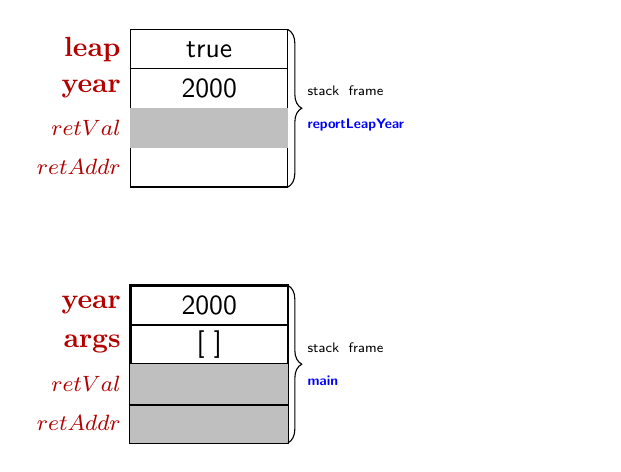
\begin{tikzpicture}[font=\sffamily, scale=0.5]
    \begin{scope}
      % Draw the stack rectangles
  \draw (0,-0.0) rectangle (4.0,-1.0);
  \draw (0,-1.0) rectangle (4.0,-2.0);
  \draw (0,-2.0) rectangle (4.0,-3.0);
  \draw (0,-3.0) rectangle (4.0,-4.0);

  % Fill gray areas
  \fill[gray!50] (0,-2.0) rectangle (4.0,-3.0);

  % Labels inside rectangles
  \node at (2.0,-0.5) {true};
  \node at (2.0,-1.5) {2000};
  \node at (2.0,-2.5) {};
  \node at (2.0,-3.5) {};

  % Variable names on left
  \node[anchor=east, text=red!70!black, font=\bfseries] at (0,-0.5) {leap};
  \node[anchor=east, text=red!70!black, font=\bfseries] at (0,-1.5) {year};
  \node[anchor=east, text=red!70!black, font=\bfseries] at (0,-2.5) {\footnotesize $retVal$};
  \node[anchor=east, text=red!70!black, font=\bfseries] at (0,-3.5) {\footnotesize $retAddr$};

  % Bracket for annotation
  \draw[decorate,decoration={brace,amplitude=5pt,mirror}]
    (4.0,-4.0) -- (4.0,0) node[midway,xshift=2cm,text width=3.5cm,align=left]
    {\tiny stack frame \\ \textit{\textbf{\textcolor{blue}{reportLeapYear}}}};
  \end{scope}

  % Second picture shifted down by 0.5 cm
  \begin{scope}[yshift=-6.5cm] % radius 1cm + 0.5cm gap
    % Draw the stack rectangles
  \draw[thick] (0,0.0) rectangle (4.0,-1.0);
  \draw[thick] (0,-1.0) rectangle (4.0,-2.0);
  \draw[thick] (0,-2.0) rectangle (4.0,-3.0);
  \draw[thick] (0,-3.05) rectangle (4.0,-4.0);

  % Fill gray areas
  \fill[gray!50] (0,-2.0) rectangle (4.0,-3.0);
  \fill[gray!50] (0,-3.05) rectangle (4.0,-4.0);

  % Labels inside rectangles
  \node at (2.0,-0.5) {2000};
  \node at (2.0,-1.5) {[\ ]};
  \node at (2.0,-2.5) {};
  \node at (2.0,-3.5) {};

  % Variable names on left
  \node[anchor=east, text=red!70!black, font=\bfseries] at (0,-0.5) {year};
  \node[anchor=east, text=red!70!black, font=\bfseries] at (0,-1.5) {args};
  \node[anchor=east, text=red!70!black, font=\bfseries] at (0,-2.5) {\footnotesize $retVal$};
  \node[anchor=east, text=red!70!black, font=\bfseries] at (0,-3.5) {\footnotesize $retAddr$};

  % Bracket for annotation
  \draw[decorate,decoration={brace,amplitude=5pt,mirror}]
    (4.0,-4.0) -- (4.0,0) node[midway,xshift=2cm,text width=3.5cm,align=left]
    {\tiny stack frame \\ \textit{\textbf{\textcolor{blue}{main}}} };
  \end{scope}
    % \
      
    \end{tikzpicture}
\end{columns}
\vspace{1cm}

\end{frame}














































% slide 6
\begin{frame}[fragile]{\texttt{reportLeapYear}:L7 affichage d'un message avec \texttt{System.out.println}}
\begin{columns}[T]
    % Left column: Code with spotlight
    \column{0.63\textwidth}
    \begin{tikzpicture}
        % Code listing (named node so we can reference its bounds)
        \node[anchor=north west] (code) at (0,0) {
            \begin{minipage}{\textwidth}
   \begin{lstlisting}[style=JavaStyle,firstnumber=1]
public class LeapYear {
    static boolean isLeap(int year) {
        return (year % 4 == 0) && (year % 100 != 0) || (year % 400 == 0);
    }
    static void reportLeapYear(int year) {
        boolean leap = isLeap(year);
        System.out.println("isLeap(" + year + ")=" + leap);
    }
    public static void main(String[] args) {
        int year = 2000;
        reportLeapYear(year);
    }
}
    \end{lstlisting}
            \end{minipage}
        };
        
        % === Spotlight the current line: draw a semi-opaque overlay with a hole ===
        \begin{scope}[on background layer]
            % Compute a window rectangle around the current line
            \path let \p1=(code.north west), \p2=(code.north east) in
                coordinate (winNW) at (\x1, \y1-6.0em)  % top-left of the window
                coordinate (winSE) at (\x2, \y1-5.3em); % bottom-right of the window
            
            % Wash out (pseudo-blur) everything except the window using even-odd rule
            \fill[black,opacity=0.3,even odd rule]
                ([yshift=0.34cm]code.south west) rectangle ([yshift=-0.27cm]code.north east)
                (winNW) rectangle (winSE);
            
            % Draw the red box around the visible line
            \draw[red,very thick,rounded corners=2pt] (winNW) rectangle (winSE);
        \end{scope}
    \end{tikzpicture}
    
    % Right column: Stack diagram
    \column{0.32\textwidth}
      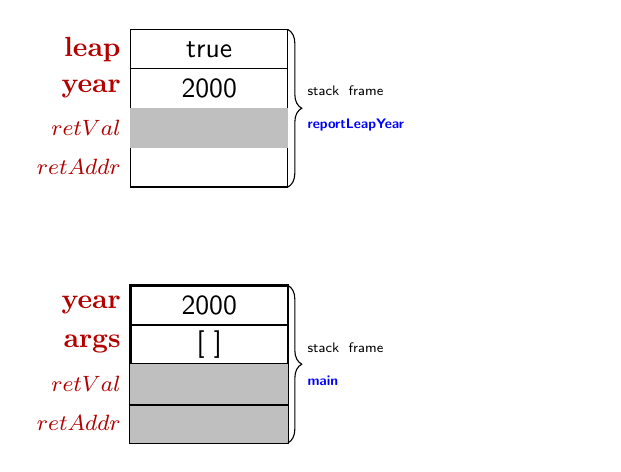
\begin{tikzpicture}[font=\sffamily, scale=0.5]
    \begin{scope}
      % Draw the stack rectangles
  \draw (0,-0.0) rectangle (4.0,-1.0);
  \draw (0,-1.0) rectangle (4.0,-2.0);
  \draw (0,-2.0) rectangle (4.0,-3.0);
  \draw (0,-3.0) rectangle (4.0,-4.0);

  % Fill gray areas
  \fill[gray!50] (0,-2.0) rectangle (4.0,-3.0);

  % Labels inside rectangles
  \node at (2.0,-0.5) {true};
  \node at (2.0,-1.5) {2000};
  \node at (2.0,-2.5) {};
  \node at (2.0,-3.5) {};

  % Variable names on left
  \node[anchor=east, text=red!70!black, font=\bfseries] at (0,-0.5) {leap};
  \node[anchor=east, text=red!70!black, font=\bfseries] at (0,-1.5) {year};
  \node[anchor=east, text=red!70!black, font=\bfseries] at (0,-2.5) {\footnotesize $retVal$};
  \node[anchor=east, text=red!70!black, font=\bfseries] at (0,-3.5) {\footnotesize $retAddr$};

  % Bracket for annotation
  \draw[decorate,decoration={brace,amplitude=5pt,mirror}]
    (4.0,-4.0) -- (4.0,0) node[midway,xshift=2cm,text width=3.5cm,align=left]
    {\tiny stack frame \\ \textit{\textbf{\textcolor{blue}{reportLeapYear}}}};
  \end{scope}

  % Second picture shifted down by 0.5 cm
  \begin{scope}[yshift=-6.5cm] % radius 1cm + 0.5cm gap
    % Draw the stack rectangles
  \draw[thick] (0,0.0) rectangle (4.0,-1.0);
  \draw[thick] (0,-1.0) rectangle (4.0,-2.0);
  \draw[thick] (0,-2.0) rectangle (4.0,-3.0);
  \draw[thick] (0,-3.05) rectangle (4.0,-4.0);

  % Fill gray areas
  \fill[gray!50] (0,-2.0) rectangle (4.0,-3.0);
  \fill[gray!50] (0,-3.05) rectangle (4.0,-4.0);

  % Labels inside rectangles
  \node at (2.0,-0.5) {2000};
  \node at (2.0,-1.5) {[\ ]};
  \node at (2.0,-2.5) {};
  \node at (2.0,-3.5) {};

  % Variable names on left
  \node[anchor=east, text=red!70!black, font=\bfseries] at (0,-0.5) {year};
  \node[anchor=east, text=red!70!black, font=\bfseries] at (0,-1.5) {args};
  \node[anchor=east, text=red!70!black, font=\bfseries] at (0,-2.5) {\footnotesize $retVal$};
  \node[anchor=east, text=red!70!black, font=\bfseries] at (0,-3.5) {\footnotesize $retAddr$};

  % Bracket for annotation
  \draw[decorate,decoration={brace,amplitude=5pt,mirror}]
    (4.0,-4.0) -- (4.0,0) node[midway,xshift=2cm,text width=3.5cm,align=left]
    {\tiny stack frame \\ \textit{\textbf{\textcolor{blue}{main}}} };
  \end{scope}
    % \
      
    \end{tikzpicture}
\end{columns}
\vspace{1cm}

\end{frame}





















\begin{frame}[fragile]{\texttt{reportLeapYear}:L7 sortie de la méthode \texttt{reportLeapYear}}
\begin{columns}[T]
    % Left column: Code with spotlight
    \column{0.63\textwidth}
    \begin{tikzpicture}
        % Code listing (named node so we can reference its bounds)
        \node[anchor=north west] (code) at (0,0) {
            \begin{minipage}{\textwidth}
   \begin{lstlisting}[style=JavaStyle,firstnumber=1]
public class LeapYear {
    static boolean isLeap(int year) {
        return (year % 4 == 0) && (year % 100 != 0) || (year % 400 == 0);
    }
    static void reportLeapYear(int year) {
        boolean leap = isLeap(year);
        System.out.println("isLeap(" + year + ")=" + leap);
    }
    public static void main(String[] args) {
        int year = 2000;
        reportLeapYear(year);
    }
}
    \end{lstlisting}
            \end{minipage}
        };
        
        % === Spotlight the current line: draw a semi-opaque overlay with a hole ===
        \begin{scope}[on background layer]
            % Compute a window rectangle around the current line
            \path let \p1=(code.north west), \p2=(code.north east) in
                coordinate (winNW) at (\x1, \y1-6.1em)  % top-left of the window
                coordinate (winSE) at (\x2, \y1-5.3em); % bottom-right of the window
            
            % Wash out (pseudo-blur) everything except the window using even-odd rule
            \fill[black,opacity=0.3,even odd rule]
                ([yshift=0.34cm]code.south west) rectangle ([yshift=-0.27cm]code.north east)
                (winNW) rectangle (winSE);
            
            % Draw the red box around the visible line
            \draw[red,very thick,rounded corners=2pt] (winNW) rectangle (winSE);
        \end{scope}
    \end{tikzpicture}
    
    % Right column: Stack diagram
    \column{0.32\textwidth}
    \vspace{0.5cm}
      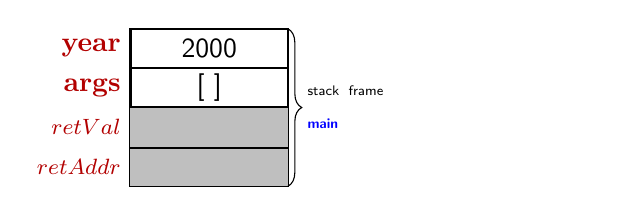
\begin{tikzpicture}[font=\sffamily, scale=0.5]
    

  % Second picture shifted down by 0.5 cm
  \begin{scope} % radius 1cm + 0.5cm gap
    % Draw the stack rectangles
  \draw[thick] (0,0.0) rectangle (4.0,-1.0);
  \draw[thick] (0,-1.0) rectangle (4.0,-2.0);
  \draw[thick] (0,-2.0) rectangle (4.0,-3.0);
  \draw[thick] (0,-3.05) rectangle (4.0,-4.0);

  % Fill gray areas
  \fill[gray!50] (0,-2.0) rectangle (4.0,-3.0);
  \fill[gray!50] (0,-3.05) rectangle (4.0,-4.0);

  % Labels inside rectangles
  \node at (2.0,-0.5) {2000};
  \node at (2.0,-1.5) {[\ ]};
  \node at (2.0,-2.5) {};
  \node at (2.0,-3.5) {};

  % Variable names on left
  \node[anchor=east, text=red!70!black, font=\bfseries] at (0,-0.5) {year};
  \node[anchor=east, text=red!70!black, font=\bfseries] at (0,-1.5) {args};
  \node[anchor=east, text=red!70!black, font=\bfseries] at (0,-2.5) {\footnotesize $retVal$};
  \node[anchor=east, text=red!70!black, font=\bfseries] at (0,-3.5) {\footnotesize $retAddr$};

  % Bracket for annotation
  \draw[decorate,decoration={brace,amplitude=5pt,mirror}]
    (4.0,-4.0) -- (4.0,0) node[midway,xshift=2cm,text width=3.5cm,align=left]
    {\tiny stack frame \\ \textit{\textbf{\textcolor{blue}{main}}} };
  \end{scope}
    % \
      
    \end{tikzpicture}
\end{columns}
\vspace{1cm}


\end{frame}






















\begin{frame}[fragile]{\texttt{main}:L11 sortie de la méthode \texttt{main}}
\begin{columns}[T]
    % Left column: Code with spotlight
    \column{0.63\textwidth}
    \begin{tikzpicture}
        % Code listing (named node so we can reference its bounds)
        \node[anchor=north west] (code) at (0,0) {
            \begin{minipage}{\textwidth}
   \begin{lstlisting}[style=JavaStyle,firstnumber=1]
public class LeapYear {
    static boolean isLeap(int year) {
        return (year % 4 == 0) && (year % 100 != 0) || (year % 400 == 0);
    }
    static void reportLeapYear(int year) {
        boolean leap = isLeap(year);
        System.out.println("isLeap(" + year + ")=" + leap);
    }
    public static void main(String[] args) {
        int year = 2000;
        reportLeapYear(year);
    }
}
    \end{lstlisting}
            \end{minipage}
        };
        
        % === Spotlight the current line: draw a semi-opaque overlay with a hole ===
        \begin{scope}[on background layer]
            % Compute a window rectangle around the current line
            \path let \p1=(code.north west), \p2=(code.north east) in
                coordinate (winNW) at (\x1, \y1-8.6em)  % top-left of the window
                coordinate (winSE) at (\x2, \y1-7.9em); % bottom-right of the window
            
            % Wash out (pseudo-blur) everything except the window using even-odd rule
            \fill[black,opacity=0.3,even odd rule]
                ([yshift=0.34cm]code.south west) rectangle ([yshift=-0.27cm]code.north east)
                (winNW) rectangle (winSE);
            
            % Draw the red box around the visible line
            \draw[red,very thick,rounded corners=2pt] (winNW) rectangle (winSE);
        \end{scope}
    \end{tikzpicture}
    
    % Right column: Stack diagram
    \column{0.32\textwidth}
    \vspace{0.5cm}
      \begin{tikzpicture}[font=\sffamily, scale=0.5]
    

      
    \end{tikzpicture}
\end{columns}
\vspace{1cm}

\end{frame}











\begin{frame}{\faCirclePlay \ Besoin de plus de visualisations?}
    Visitez ce site-web génial pour plus de visualisations:
    \url{https://cscircles.cemc.uwaterloo.ca/java_visualize/}
\end{frame}



\end{document}
